\documentclass[11pt,letter]{article}

\usepackage[latin1]{inputenc}
\usepackage{amsmath}
\usepackage{amsfonts}
\usepackage{amssymb}
\usepackage{amsthm}
\usepackage{enumitem}
\usepackage[english]{babel}
\usepackage{fancyhdr}
\usepackage{lipsum}
\usepackage{chngpage}
\usepackage{geometry}
\usepackage{mathtools}
\usepackage{tabularx}
\usepackage{verbatim}
\usepackage{tikz}
\usepackage[ruled,vlined]{algorithm2e}
\geometry{letterpaper, portrait, margin=1in}
 
\pagestyle{fancy}
\fancyhf{}
\rhead{\thepage}
\lhead{Implementing Path 3-Coloring and Path 3-Choosing Algorithms on Plane Graphs}
\rfoot{}

\newcommand{\overbar}[1]{\mkern 1.5mu\overline{\mkern-1.5mu#1\mkern-1.5mu}\mkern 1.5mu}

\begin{document}

\title{Implementing Path 3-Coloring and Path 3-Choosing Algorithms on Plane Graphs}
\date{August 2, 2016}

\maketitle

\section*{Abstract}

Path coloring a graph partitions its vertices into sets inducing a disjoint union of paths. In this project
we consider several algorithms to compute path colorings of graphs embedded in the plane. We
first implement an algorithm path 3-color plane graphs from Poh's proof in [a]. Second, we present a linear time
implementation of an algorithm to path 3-choose plane graphs from the independant work of Hartman [b] and
Skrekovski [c].

\section{Introduction}

All graphs discussed in this project will be simple, undirected, and finite. A graph is planar if it may
be drawn in the plane without edge crossings. A $k$-coloring of a graph partitions
its vertices into $k$ color classes. Such a coloring is called proper if each color class consists of
nonadjacent vertices. In 1976 Appel and Haken [d,e] displayed that all planar graphs have a proper $4$-coloring.
This result is best possible and solved the century old Four Color Conjecture.
Generalizations of proper coloring were introduced in [f,g,h] allowing color classes to form forests, or allowing vertices
to have some bounded number of same color neighbors. Cowen et al. ([j]) show a best possible result that planar
graphs may be $3$-colored such that each vertex recieves at most two same color neighbors.\\

\noindent We will be considering the problem of path coloring, producing a $k$-coloring of a graph such that each color
class induces a disjoint union of paths, or equivalently a forest where each component is a path. This coloring
was introduced by Harary in [i]. Note that this is similar to the defective coloring of Cowen et al. above,
with the added restriction that path coloring forbids cycles. In [l] Poh displayes that all
planar graphs have a path $3$-coloring. Here we present an implementation of Poh's algorithm to path
$3$-color plane graphs.\\

\noindent Given a list of $k$ colors for each vertex, a $k$-list-coloring assigns each vertex a color from its list.
If a graph has a proper $k$-list-coloring it is said to be $k$-choosable. List-coloring was first introduced by
Erd{\"o}s et al. in [m]. Thomassen in [n] proves that all planar graphs are $5$ choosable. Planar
graphs that are not $4$-choosable are described by Mirzakhani in [o] and Voigt in [p], so Thomassen's result
is best possible.\\

\noindent Hull and Eaton in [q] prove planar graphs are $3$-choosable such that each vertex recieves at most two
same color neighbors, and furthermore show this result is best possible. Hartman in [r] and Skrekovski in [s] independantly
provide similar proofs that planar graphs are path $3$-choosable. Hartman claims the proof yields
a linear time algorithm for path $3$-list-coloring, and thus path $3$-coloring, plane graphs. Here we present a
linear time implementation of Hartman and Skrekovski's algorithm.\\

\section{Path $3$-Coloring Plane Graphs}

We first restate the algorithm and proof of Poh [l] for path $3$-coloring plane graphs.\\

\begin{adjustwidth}{1.5em}{1.5em}
\noindent\textbf{Theorem 1.} Let $G$ be a $2$-connected weakly triangulated plane graph and
suppose the outer face $C$ has been $2$-colored such that each color class induces a non-empty path. This
$2$-coloring may be extended to a path $3$-coloring of $G$ such that no vertex in $C$ recieves a same color
neighbor.
\end{adjustwidth}

\begin{proof}
\noindent Let $P=p_0\ldots p_n$ and $Q=q_0\ldots q_m$ denote the two induced paths from the $2$-coloring of $C$
such that the edges $p_0q_0$ and $p_nq_m$ are in $C$. Suppose there exist uncolored vertices, that is
$V(G)\setminus V(C)\ne\emptyset$.\\

\noindent Let $t_0$ be the vertex forming a face with $p_0$ and $q_0$. If $t_0\in P$, this face is already
colored and we consider the graph bounded by $P-p_0$ and $Q$. Similarly, if $t_0\in Q$ we consider
the graph bounded by $P$ and $Q-q_0$. Let $t_1$ be the vertex forming a face with $p_n$ and $q_m$ and
proceed in the same manner until $t_1$ is not in either path.\\

\noindent Suppose there exists an induced path $T$ from $t_0$ to $t_1$. We color $T$ the remaining color not
assigned to $P$ or $Q$ and now separately consider the subgraph bounded by $P$ and $T$, and the subgraph bounded
by $T$ and $Q$.\\

\noindent Suppose no path exists from $t_0$ to $t_1$. Then for some $p_i\in P$ and $q_j\in Q$, there exists an
edge $p_iq_m$. We then separately consider the subgraph bounded by $p_0\ldots p_i$ and $q_0\ldots q_j$, and
the subgraph bounded by $p_i\ldots p_n$ and $q_j\ldots q_m$.
\end{proof}

\subsection*{Implementation}

Let the plane graph $G$ be represented as an adjacency list and an ordering of neighbors following a
combinatorial embedding. We track the paths $P$ and $Q$ by marking each path vertex and storing the endpoints
of the paths. To find $t_0$ we look at the ordered neighbors of $p_0$ and take the vertex clockwise past $q_0$.
We find $t_1$ similarly by looking at $p_n$ and $q_m$.\\

\noindent To check for the path from $t_0$ to $t_1$ we perform a
breadth first search starting at $t_1$, and store parents for each vertex visited. If $t_0$ is reached, an induced path from $t_0$ 
to $t_1$ is produced by backtracking through the search. We then color and mark each vertex on the new path.
Otherwise, we find a vertex $u$ with consecutive neighbors in opposite paths. These vertices
will be $p_i$ and $q_j$. We may then immediately recurse on region bounded by the $p_ip_n$-path and $ut_1$-path
and the region bounded by the $ut_1$-path and the $q_jp_m$-path. To handle the remaining graph we also recurse
using the $p_0p_i$-path and $q_0p_j$-path.\\

\begin{center}
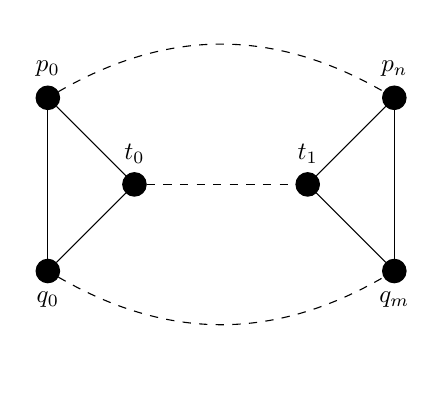
\begin{tikzpicture}[
		scale=1.1,
		every node/.style={circle, draw, minimum size=1mm, scale=0.9},
		every label/.append style={rectangle}
	]
  \node (p0) [label=above:$p_0$, fill] at (-2cm, 1cm) {};
  \node (pn) [label=above:$p_n$, fill] at (2cm, 1cm) {};
  \node (q0) [label=below:$q_0$, fill] at (-2cm, -1cm) {};
  \node (qn) [label=below:$q_m$, fill] at (2cm, -1cm) {};
  \node (t0) [label=above:$t_0$, fill] at (-1cm, 0cm) {};
  \node (t1) [label=above:$t_1$, fill] at (1cm, 0cm) {};
  \node (null) [draw=none] at (270:2cm) {};
  \draw (p0) edge [bend left] (pn) [dashed];
  \draw (q0) edge [bend right] (qn) [dashed];
  \draw (p0) edge (q0);
  \draw (pn) edge (qn);
  \draw (p0) edge (t0);
  \draw (q0) edge (t0);
  \draw (pn) edge (t1);
  \draw (qn) edge (t1);
  \draw (t0) edge (t1) [dashed];
\end{tikzpicture}
$\qquad$
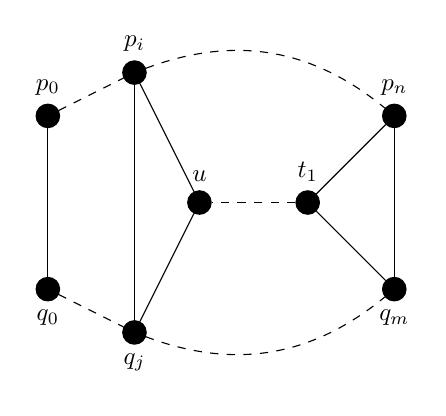
\begin{tikzpicture}[
		scale=1.1,
		every node/.style={circle, draw, minimum size=1mm, scale=0.9},
		every label/.append style={rectangle}
	]
  \node (p0) [label=above:$p_0$, fill] at (-2cm, 1cm) {};
  \node (pn) [label=above:$p_n$, fill] at (2cm, 1cm) {};
  \node (q0) [label=below:$q_0$, fill] at (-2cm, -1cm) {};
  \node (qn) [label=below:$q_m$, fill] at (2cm, -1cm) {};
  \node (t0) [label=above:$u$, fill] at (-0.25cm, 0cm) {};
  \node (t1) [label=above:$t_1$, fill] at (1cm, 0cm) {};
  \node (pi) [label=above:$p_i$, fill] at (-1cm, 1.5cm) {};
  \node (qj) [label=below:$q_j$, fill] at (-1cm, -1.5cm) {};
  \node (null) [draw=none] at (270:2cm) {};
  \draw (p0) edge (pi) [dashed];
  \draw (pi) edge [bend left] (pn) [dashed];
  \draw (q0) edge (qj) [dashed];
  \draw (qj) edge [bend right] (qn) [dashed];
  \draw (p0) edge (q0);
  \draw (pn) edge (qn);
  \draw (pi) edge (qj);
  \draw (pn) edge (t1);
  \draw (qn) edge (t1);
  \draw (t1) edge (t0) [dashed];
  \draw (pi) edge (t0);
  \draw (qj) edge (t0);
\end{tikzpicture}
\hfill\\
\footnotesize{\textbf{Figure 2.1} The case of a $t_0t_1$ path (left) and the case of a an ede $p_ip_j$ (right).}
\end{center}

\noindent In locating $t_0$ and $t_1$ we make a neighbor lookup once for each. The amortized complexity of a
neighbor lookup is $O(|E|/|V|)$. Since a vertex may only be $t_0$
or $t_1$ once in the algorithm, we perform at most $|V|$ neighbor lookups, and the total amoritized complexity
of this step is $O(|V||E|/|V|)=O(|E|)$. In planar graphs $|E|\le 3|V|-6$, and $O(|E|)=O(|V|)$. Therefore, the
amortized complexity of this step over the entire graph is $O(|V|)$. We also perform at most one breadth first
search from each $t_1$, each with complexity $O(|V|)$. Therefore the complexity of the serach step over the
entire graph is $O(|V|^2)$. This gives us an overall amortized complexity of $O(|V|+|V|^2)=O(|V|^2)$.

\section{Path $3$-Choosing Plane Graphs}

The following theorem is a significant restatement of the work of Hartman [r] and Skrekovski [s]. Suppose $C$ is
the outer cycle of a weakly triangulated plane graph $G$. Using notation from [r] for vertices $u,v\in C$ we
let $C[u,v]$ denote the path from $u$ to $v$ clockwise along the outer face. Similarly, for $v\in V(G)$ and
$u,w\in N(v)$ we let $[u,w]_v$ denote the path from $u$ to $w$ clockwise around $v$, assuming triangulated
faces.\\

\begin{adjustwidth}{1.5em}{1.5em}
\noindent\textbf{Theorem 2.} Let $G$ be a $2$-connected weakly triangulated plane graph with outer face $C$, or
a complete graph on two vertices.
Let $x,y\in C$ be not necessarily distinct, potentially precolored vertices. Suppose $L(v)$ assigns a list of colors to each $v\in V(G)$ such that
\[
    \begin{array}{ll}
	    |L(v)|\ge 1 & \text{if } v=x \text{ or } v=y \text{ or } v=p;\\
	    |L(v)|\ge 2 & \text{if } v\in C, v\ne x, v\ne y;\\
	    |L(v)|\ge 3 & \text{otherwise.}
    \end{array}
\]
Let $p\in C[x,y]$ be precolored some color $\alpha\in L(p)$. If $p\ne x$, suppose $\alpha\not\in L(v)$ for
any $v\in C[x,p)$.\\

\noindent The coloring may then be extended to
a path choosing of $G$ from $L$ such that $x$, $y$, and $p$ recieve at most one same color neighbor. If
$x=y$ then $x$ and $y$ recieve no same color neighbors. If $y=p$, or $y$ is immediately prior to
$p$ on the outer face and $\alpha\not\in L(y)$, then $y$ recieves no same color neighbors.\\
\end{adjustwidth}

\begin{proof}
Suppose $|V(G)|=2$. If $x=y=p$ color the remaining vertex any color in its list other than $\alpha$. Otherwise,
color the remaining color any color in its list if it has not been precolored.\\

\noindent Suppose $|V(G)|>2$ and the theorem holds for all graphs $H$ with $|V(H)|<|V(G)|$. Let
$C=c_0c_1\ldots c_n$ denote, in clockwise order, the outer face of $G$ with $p=c_0$.
There are several cases to consider. Let $c_i\in C$ be the next neighhbor of $p$ counterclockwise from $c_n$.
Let $G_0$ be the subgraph bounded by the cycle formed from $C[c_i,c_n]$ and $[c_n,c_i]_p$. If $c_i\ne c_1$ let
$G_1$ be the sugbraph bounded by the cycle formed from $C[p,c_i]$ and the edge $pc_i$. As seen in Figure
3.1 $G=G_0\cup G_1$
and $V(G_0)\cap V(G_1)=\{c_i\}$.
We will display in each case that the inductive hypothesis holds for each subgraph and show their union still
forms a path choosing of $G$ from $L$.
If $c_i=c_1$ then $G_1$ will not exist and we handle this case specially, noting $G_0=G-p$.\\

\noindent Note that in all figures solid circles denote vertices yet to be colored, and colored vertices will
be labeled with their assigned color. A label $\beta$ will denote a color distinct from $\alpha$. If a vertex
is unlabled it represents arbitrary color assignment from $L$.

\begin{center}
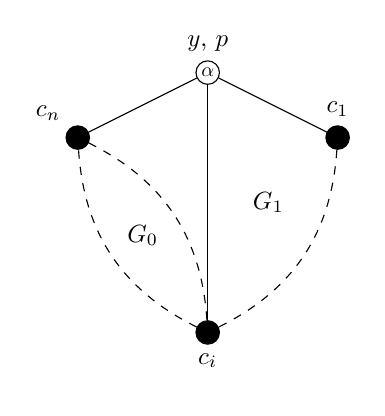
\begin{tikzpicture}[
		scale=1.1,
		every node/.style={circle, draw, minimum size=1mm, scale=0.9},
		every label/.append style={rectangle}
	]
  \node (c_n) [label=above left:$c_n$, fill] at (-1.5cm, 1.25cm) {};
  \node (p) [label=above:{$y$, $p$}] at (0cm, 2cm) {};
  \node (p_label) [draw=none, scale=0.8] at (0cm, 2cm) {$\alpha$};
  \node (c_1) [label=above:$c_1$, fill] at (1.5cm, 1.25cm) {};
  \node (c_i) [label=below:$c_i$, fill] at (0cm, -1cm) {};
  \node (G_0) [draw=none, ] at (-0.75cm, 0.12cm) {$G_0$};
  \node (G_1) [draw=none] at (0.7cm, 0.5cm) {$G_1$};
  \node (null) [draw=none] at (270:1.5cm) {};
  \draw (c_i) edge [bend left] (c_n) [dashed];
  \draw (c_n) edge [bend left] (c_i) [dashed];
  \draw (c_n) edge (p);
  \draw (p) edge (c_1);
  \draw (p) edge (c_i);
  \draw (c_1) edge [bend left] (c_i) [dashed];
\end{tikzpicture}
\hfill\\
\footnotesize{\textbf{Figure 3.1} The subdivision of $G$ into $G_0$ and $G_1$.}
\end{center}

\noindent For all $v\in N(p)\cap V(G_0)\setminus\{x,y\}$ we note if $v=c_n$ or $v=c_i$
then $|L(v)|\ge 2$, and $|L(v)|\ge3$ otherwise. We define a new list assignment $L_0$
such that $L_0(v)=L(v)\setminus\{\alpha\}$ for
$v\in N(p)\cap V(G_0)$, and $L_0(v)=L(v)$ for $v\in V(G_0)\setminus N(p)$. Note that all
$v\in N(p)\cap V(G_0)$ will be on the outer face of $G_0$. Thus $|L_0(v)|\ge 3$ for all interior
vertices $v$ of $G_0$. Also, $|L_0(v)|\ge 1$ for all $v\in\{x,y,c_i,c_n\}$. The case $\alpha\in L(y)$ when
$y\in V(G_i)\cap N(p)$ will potentially result in $|L_0(y)|=0$, but in this case $y=c_i$ and $y$ will be
colored $\alpha$ in the appropriate case. Finally, $|L_0|\ge2$ for all other $v$ on the outer face of $G_0$.

\begin{center}
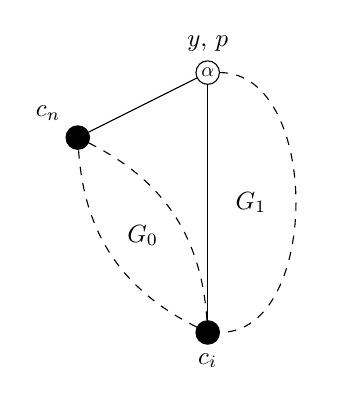
\begin{tikzpicture}[
		scale=1.1,
		every node/.style={circle, draw, minimum size=1mm, scale=0.9},
		every label/.append style={rectangle}
	]
  \node (c_n) [label=above left:$c_n$, fill] at (-1.5cm, 1.25cm) {};
  \node (p) [label=above:{$y$, $p$}] at (0cm, 2cm) {};
  \node (p_label) [draw=none, scale=0.8] at (0cm, 2cm) {$\alpha$};
  \node (c_i) [label=below:$c_i$, fill] at (0cm, -1cm) {};
  \node (G_0) [draw=none, ] at (-0.75cm, 0.12cm) {$G_0$};
  \node (G_1) [draw=none] at (0.5cm, 0.5cm) {$G_1$};
  \node (null) [draw=none] at (270:1.5cm) {};
  \draw (c_i) edge [bend left] (c_n) [dashed];
  \draw (c_n) edge [bend left] (c_i) [dashed];
  \draw (c_n) edge (p);
  \draw (p) edge (c_i);
  \draw (p) edge [bend left=90] (c_i) [dashed];
\end{tikzpicture}
$\qquad$
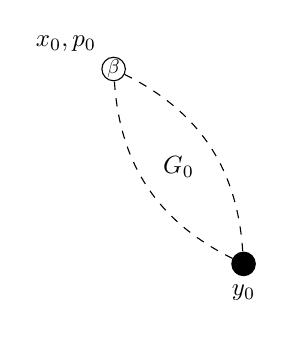
\begin{tikzpicture}[
		scale=1.1,
		every node/.style={circle, draw, minimum size=1mm, scale=0.9},
		every label/.append style={rectangle}
	]
  \node (c_n) [label=above left:{$x_0,p_0$}] at (-1.5cm, 1.25cm) {};
  \node (c_i) [label=below:$y_0$, fill] at (0cm, -1cm) {};
  \node (c_n_label) [draw=none, scale=0.8] at (-1.5cm, 1.25cm) {$\beta$};
  \node (G_0) [draw=none] at (-0.75cm, 0.12cm) {$G_0$};
  \node (null) [draw=none] at (270:1.5cm) {};
  \draw (c_i) edge [bend left] (c_n) [dashed];
  \draw (c_n) edge [bend left] (c_i) [dashed];
\end{tikzpicture}
$\qquad$
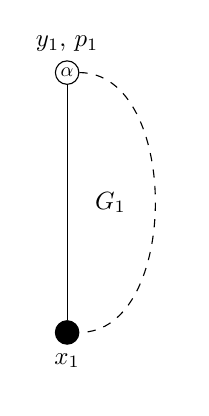
\begin{tikzpicture}[
		scale=1.1,
		every node/.style={circle, draw, minimum size=1mm, scale=0.9},
		every label/.append style={rectangle}
	]
  \node (p) [label=above:{$y_1$, $p_1$}] at (0cm, 2cm) {};
  \node (p_label) [draw=none, scale=0.8] at (0cm, 2cm) {$\alpha$};
  \node (c_i) [label=below:$x_1$, fill] at (0cm, -1cm) {};
  \node (G_1) [draw=none] at (0.5cm, 0.5cm) {$G_1$};
  \node (null) [draw=none] at (270:1.5cm) {};
  \draw (p) edge (c_i);
  \draw (p) edge [bend left=90] (c_i) [dashed];
\end{tikzpicture}
\hfill\\
\footnotesize{\textbf{Figure 3.2} The case $x=y=p$.}
\end{center}

\noindent Suppose $x=y=p$. Define $p_0=c_n$ and precolor $p_0$ from $L_0(p_0)$. By our note above, clearly
$L_0(v)$ satisfies the inductive hypothesis with $G_0$, $x_0=c_n$, $y_0c_i$, and $p_0$. After choosing $G_0$
from $L_0$, if $G_1$ exists we apply the inductive hypothesis again to choose $G_1$ from $L$ with $x_1=c_i$,
$y_1=y$, and $p_1=p$. Since $c_i$ recieves at most one neighbor in each $G_0$ and $G_1$, the combined coloring
forms a path choosing of $G$ from $L$.\\

\begin{center}
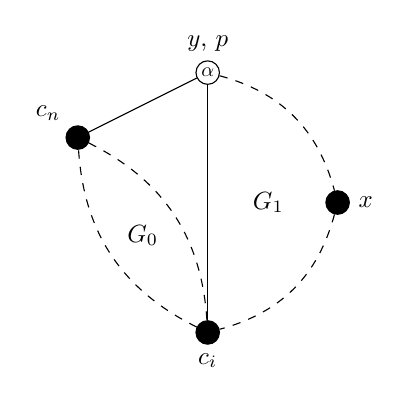
\begin{tikzpicture}[
		scale=1.1,
		every node/.style={circle, draw, minimum size=1mm, scale=0.9},
		every label/.append style={rectangle}
	]
  \node (c_n) [label=above left:$c_n$, fill] at (-1.5cm, 1.25cm) {};
  \node (p) [label=above:{$y$, $p$}] at (0cm, 2cm) {};
  \node (p_label) [draw=none, scale=0.8] at (0cm, 2cm) {$\alpha$};
  \node (x) [label=right:$x$, fill] at (1.5cm, 0.5cm) {};
  \node (c_i) [label=below:$c_i$, fill] at (0cm, -1cm) {};
  \node (G_0) [draw=none, ] at (-0.75cm, 0.12cm) {$G_0$};
  \node (G_1) [draw=none] at (0.7cm, 0.5cm) {$G_1$};
  \node (null) [draw=none] at (270:1.5cm) {};
  \draw (c_i) edge [bend left] (c_n) [dashed];
  \draw (c_n) edge [bend left] (c_i) [dashed];
  \draw (c_n) edge (p);
  \draw (p) edge (c_i);
  \draw (p) edge [bend left] (x) [dashed];
  \draw (x) edge [bend left] (c_i) [dashed];
\end{tikzpicture}
$\qquad$
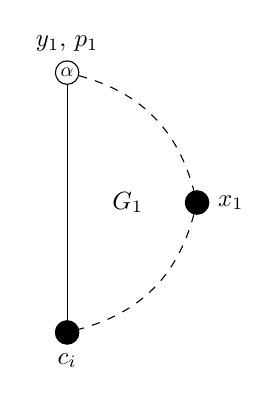
\begin{tikzpicture}[
		scale=1.1,
		every node/.style={circle, draw, minimum size=1mm, scale=0.9},
		every label/.append style={rectangle}
	]
  \node (p) [label=above:{$y_1$, $p_1$}] at (0cm, 2cm) {};
  \node (p_label) [draw=none, scale=0.8] at (0cm, 2cm) {$\alpha$};
  \node (x) [label=right:$x_1$, fill] at (1.5cm, 0.5cm) {};
  \node (c_i) [label=below:$c_i$,fill] at (0cm, -1cm) {};
  \node (G_1) [draw=none] at (0.7cm, 0.5cm) {$G_1$};
  \node (null) [draw=none] at (270:1.5cm) {};
  \draw (p) edge (c_i);
  \draw (p) edge [bend left] (x) [dashed];
  \draw (x) edge [bend left] (c_i) [dashed];
\end{tikzpicture}
$\qquad$
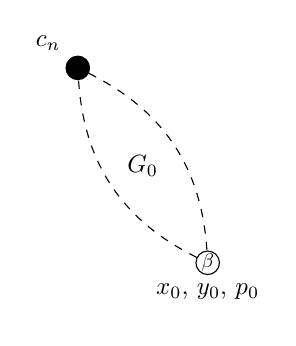
\begin{tikzpicture}[
		scale=1.1,
		every node/.style={circle, draw, minimum size=1mm, scale=0.9},
		every label/.append style={rectangle}
	]
  \node (c_n) [label=above left:{$c_n$}, fill] at (-1.5cm, 1.25cm) {};
  \node (c_i) [label=below:{$x_0$, $y_0$, $p_0$}] at (0cm, -1cm) {};
  \node (c_i_label) [draw=none, scale=0.8] at (0cm, -1cm) {$\beta$};
  \node (G_0) [draw=none] at (-0.75cm, 0.12cm) {$G_0$};
  \node (null) [draw=none] at (270:1.5cm) {};
  \draw (c_i) edge [bend left] (c_n) [dashed];
  \draw (c_n) edge [bend left] (c_i) [dashed];
\end{tikzpicture}
\hfill\\
\footnotesize{\textbf{Figure 3.3} The case $y=p$, $x\ne p$, and $c_i\in C[x,p)$.}
\end{center}

\noindent Suppose $y=p$, $x\ne p$, and $c_i\in C[x,p)$. In this case $G_1$ must exist, so first apply
the inductive hypothesis to choose $G_1$ from $L$ with $x_1=x$, $y_1=y$, and $p_1=p$.
Since $\alpha\not\in L(v)$ for any $v\in C[x,p)$ we may apply the inductive hypothesis to choose $G_0$ from
$L_0$ with $x_0=y_0=p_0=c_i$. Note that $c_i$ was precolored from our choosing of $G_1$ and recieves
no same color neighbors in $G_0$ so the combined coloring forms a path choosing of $G$ from $L$.\\

\begin{center}
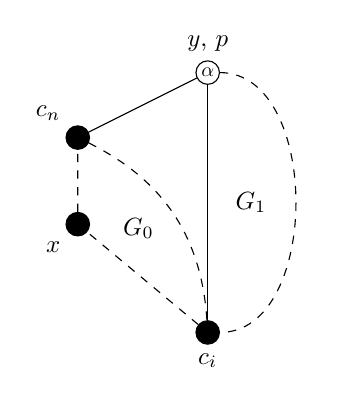
\begin{tikzpicture}[
		scale=1.1,
		every node/.style={circle, draw, minimum size=1mm, scale=0.9},
		every label/.append style={rectangle}
	]
  \node (c_n) [label=above left:$c_n$, fill] at (-1.5cm, 1.25cm) {};
  \node (p) [label=above:{$y$, $p$}] at (0cm, 2cm) {};
  \node (p_label) [draw=none, scale=0.8] at (0cm, 2cm) {$\alpha$};
  \node (x) [label=below left:$x$, fill] at (-1.5cm, 0.25cm) {};
  \node (c_i) [label=below:$c_i$, fill] at (0cm, -1cm) {};
  \node (G_0) [draw=none, ] at (-0.8cm, 0.2cm) {$G_0$};
  \node (G_1) [draw=none] at (0.5cm, 0.5cm) {$G_1$};
  \node (null) [draw=none] at (270:1.5cm) {};
  \draw (c_i) edge (x) [dashed];
  \draw (x) edge (c_n) [dashed];
  \draw (c_n) edge [bend left] (c_i) [dashed];
  \draw (c_n) edge (p);
  \draw (p) edge (c_i);
  \draw (p) edge [bend left=90] (c_i) [dashed];
\end{tikzpicture}
$\qquad$
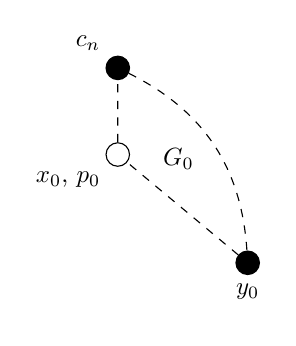
\begin{tikzpicture}[
		scale=1.1,
		every node/.style={circle, draw, minimum size=1mm, scale=0.9},
		every label/.append style={rectangle}
	]
  \node (c_n) [label=above left:$c_n$, fill] at (-1.5cm, 1.25cm) {};
  \node (x) [label=below left:{$x_0$, $p_0$}] at (-1.5cm, 0.25cm) {};
  \node (c_i) [label=below:$y_0$, fill] at (0cm, -1cm) {};
  \node (G_0) [draw=none, ] at (-0.8cm, 0.2cm) {$G_0$};
  \node (null) [draw=none] at (270:1.5cm) {};
  \draw (c_i) edge (x) [dashed];
  \draw (x) edge (c_n) [dashed];
  \draw (c_n) edge [bend left] (c_i) [dashed];
\end{tikzpicture}
$\qquad$
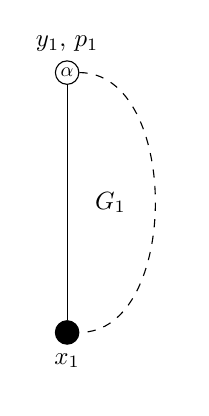
\begin{tikzpicture}[
		scale=1.1,
		every node/.style={circle, draw, minimum size=1mm, scale=0.9},
		every label/.append style={rectangle}
	]
  \node (p) [label=above:{$y_1$, $p_1$}] at (0cm, 2cm) {};
  \node (p_label) [draw=none, scale=0.8] at (0cm, 2cm) {$\alpha$};
  \node (c_i) [label=below:$x_1$, fill] at (0cm, -1cm) {};
  \node (G_1) [draw=none] at (0.5cm, 0.5cm) {$G_1$};
  \node (null) [draw=none] at (270:1.5cm) {};
  \draw (p) edge (c_i);
  \draw (p) edge [bend left=90] (c_i) [dashed];
\end{tikzpicture}
\hfill\\
\footnotesize{\textbf{Figure 3.4} The case $y=p$, $x\ne p$, and $c_i\not\in C[x,p)$.}
\end{center}

\noindent Suppose $y=p$, $x\ne p$, and $c_i\not\in C[x,p)$. Since $\alpha\not\in L(v)$
for any $v\in C[x,p)$ we color $x$ with the first color in $L_0(x)$ and apply the inductive hypothesis to choose
$G_0$ from $L_0$ with $x_0=p_0=x$ and $y_0=c_i$. If $G_1$ exists we apply the inductive hypothesis again to
choose $G_1$ from $L$ with $x_1=c_i$, $y_1=y$, and $p_1=p$. Notice $c_i$ recieves at most one same color
neighbor in each $G_0$ and $G_1$.\\

\begin{center}
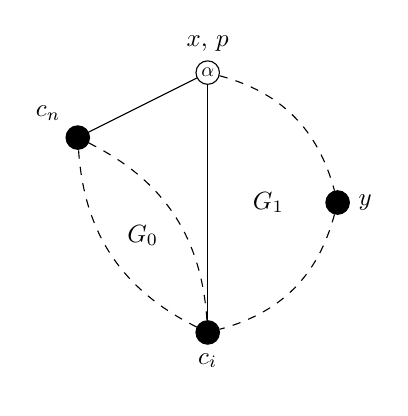
\begin{tikzpicture}[
		scale=1.1,
		every node/.style={circle, draw, minimum size=1mm, scale=0.9},
		every label/.append style={rectangle}
	]
  \node (c_n) [label=above left:$c_n$, fill] at (-1.5cm, 1.25cm) {};
  \node (p) [label=above:{$x$, $p$}] at (0cm, 2cm) {};
  \node (p_label) [draw=none, scale=0.8] at (0cm, 2cm) {$\alpha$};
  \node (y) [label=right:$y$, fill] at (1.5cm, 0.5cm) {};
  \node (c_i) [label=below:$c_i$, fill] at (0cm, -1cm) {};
  \node (G_0) [draw=none, ] at (-0.75cm, 0.12cm) {$G_0$};
  \node (G_1) [draw=none] at (0.7cm, 0.5cm) {$G_1$};
  \node (null) [draw=none] at (270:1.5cm) {};
  \draw (c_i) edge [bend left] (c_n) [dashed];
  \draw (c_n) edge [bend left] (c_i) [dashed];
  \draw (c_n) edge (p);
  \draw (p) edge (c_i);
  \draw (p) edge [bend left] (y) [dashed];
  \draw (y) edge [bend left] (c_i) [dashed];
\end{tikzpicture}
$\qquad$
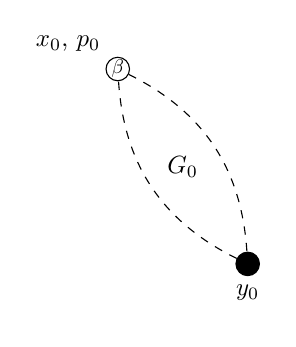
\begin{tikzpicture}[
		scale=1.1,
		every node/.style={circle, draw, minimum size=1mm, scale=0.9},
		every label/.append style={rectangle}
	]
  \node (c_n) [label=above left:{$x_0$, $p_0$}] at (-1.5cm, 1.25cm) {};
  \node (c_n_label) [draw=none, scale=0.8] at (-1.5cm, 1.25cm) {$\beta$};
  \node (c_i) [label=below:{$y_0$}, fill] at (0cm, -1cm) {};
  \node (G_0) [draw=none] at (-0.75cm, 0.12cm) {$G_0$};
  \node (null) [draw=none] at (270:1.5cm) {};
  \draw (c_i) edge [bend left] (c_n) [dashed];
  \draw (c_n) edge [bend left] (c_i) [dashed];
\end{tikzpicture}
$\qquad$
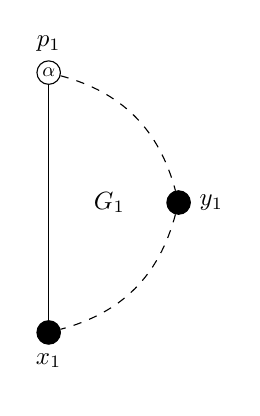
\begin{tikzpicture}[
		scale=1.1,
		every node/.style={circle, draw, minimum size=1mm, scale=0.9},
		every label/.append style={rectangle}
	]
  \node (p) [label=above:$p_1$] at (0cm, 2cm) {};
  \node (p_label) [draw=none, scale=0.8] at (0cm, 2cm) {$\alpha$};
  \node (y) [label=right:$y_1$, fill] at (1.5cm, 0.5cm) {};
  \node (c_i) [label=below:$x_1$,fill] at (0cm, -1cm) {};
  \node (G_1) [draw=none] at (0.7cm, 0.5cm) {$G_1$};
  \node (null) [draw=none] at (270:1.5cm) {};
  \draw (p) edge (c_i);
  \draw (p) edge [bend left] (y) [dashed];
  \draw (y) edge [bend left] (c_i) [dashed];
\end{tikzpicture}
\hfill\\
\footnotesize{\textbf{Figure 3.5} The case $x=p$, $y\ne p$, and $c_i\in C(y,x)$.}
\end{center}

\noindent Suppose $x=p$, $y\ne p$, and $c_i\in C(y,x)$. In this case $G_1$ must exist, so first apply the
inductive hypothesis to choose $G_0$ from $L_0$ with $x_0=p_0=c_n$ and $y_0=c_i$. We again apply the inductive
hypothesis to choose $G_1$ from $L$ with $x_1=c_i$, $y_1=y$, and $p_1=p$. Notice $c_i$ recieves at most one same
color neighbor in each $G_0$ and $G_1$.\\

\begin{center}
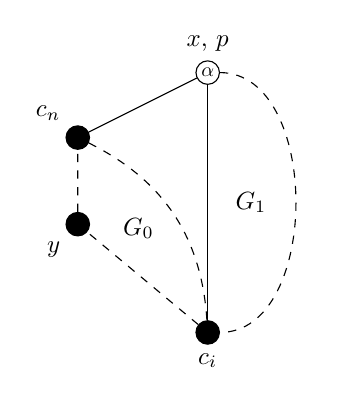
\begin{tikzpicture}[
		scale=1.1,
		every node/.style={circle, draw, minimum size=1mm, scale=0.9},
		every label/.append style={rectangle}
	]
  \node (c_n) [label=above left:$c_n$, fill] at (-1.5cm, 1.25cm) {};
  \node (p) [label=above:{$x$, $p$}] at (0cm, 2cm) {};
  \node (p_label) [draw=none, scale=0.8] at (0cm, 2cm) {$\alpha$};
  \node (y) [label=below left:$y$, fill] at (-1.5cm, 0.25cm) {};
  \node (c_i) [label=below:$c_i$, fill] at (0cm, -1cm) {};
  \node (G_0) [draw=none, ] at (-0.8cm, 0.2cm) {$G_0$};
  \node (G_1) [draw=none] at (0.5cm, 0.5cm) {$G_1$};
  \node (null) [draw=none] at (270:1.5cm) {};
  \draw (c_i) edge (y) [dashed];
  \draw (y) edge (c_n) [dashed];
  \draw (c_n) edge [bend left] (c_i) [dashed];
  \draw (c_n) edge (p);
  \draw (p) edge (c_i);
  \draw (p) edge [bend left=90] (c_i) [dashed];
\end{tikzpicture}
$\qquad$
\begin{tikzpicture}[
		scale=1.1,
		every node/.style={circle, draw, minimum size=1mm, scale=0.9},
		every label/.append style={rectangle}
	]
  \node (p) [label=above:{$x_1$, $p_1$}] at (0cm, 2cm) {};
  \node (p_label) [draw=none, scale=0.8] at (0cm, 2cm) {$\alpha$};
  \node (c_i) [label=below:$y_1$] at (0cm, -1cm) {};
  \node (c_i_label) [draw=none, scale=0.8] at (0cm, -1cm) {$\alpha$};
  \node (G_1) [draw=none] at (0.5cm, 0.5cm) {$G_1$};
  \node (null) [draw=none] at (270:1.5cm) {};
  \draw (p) edge (c_i);
  \draw (p) edge [bend left=90] (c_i) [dashed];
\end{tikzpicture}
$\qquad$
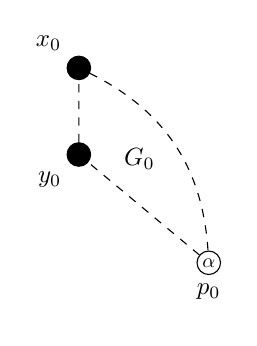
\begin{tikzpicture}[
		scale=1.1,
		every node/.style={circle, draw, minimum size=1mm, scale=0.9},
		every label/.append style={rectangle}
	]
  \node (c_n) [label=above left:$x_0$, fill] at (-1.5cm, 1.25cm) {};
  \node (y) [label=below left:$y_0$, fill] at (-1.5cm, 0.25cm) {};
  \node (c_i) [label=below:$p_0$] at (0cm, -1cm) {};
  \node (c_i_label) [draw=none, scale=0.8] at (0cm, -1cm) {$\alpha$};
  \node (G_0) [draw=none, ] at (-0.8cm, 0.2cm) {$G_0$};
  \node (null) [draw=none] at (270:1.5cm) {};
  \draw (c_i) edge (y) [dashed];
  \draw (y) edge (c_n) [dashed];
  \draw (c_n) edge [bend left] (c_i) [dashed];
\end{tikzpicture}
\hfill\\
\footnotesize{\textbf{Figure 3.6} The case $x=p$, $y\ne p$, and $c_i\not\in C(y,x)$ where $\alpha\in L(c_i)$.}
\end{center}

\noindent Suppose $x=p$, $y\ne p$, and $c_i\not\in C(y,x)$. If
$\alpha\in L(c_i)$ we set $p_0=c_i$ and color $c_i$ with $\alpha$. Otherwise, set $p_0=c_n$ and color it with
the first color in $L_0(c_n)$, note $|L_0(c_i)|\ge 2$ in this case. We then apply the inductive hypothesis to
choose $G_0$ from $L_0$ with $x_0=c_n$, $y_0=y$, and $p_0$. If $G_1$ exists, we again apply the inductive
hypothesis to color $G_1$ with $x_1=p_1=p$ and $y_1=c_i$. Notice if $p_0=c_i$, $c_i$ recieves at most one same
color neighbor in each $G_0$ and $G_1$. If $p_0\ne c_i$, then $y_1=c_i$ is immediatley prior to
$p_1=p$ and thus $c_i$ will recieve no same color neighbors in $G_1$.\\

\begin{center}
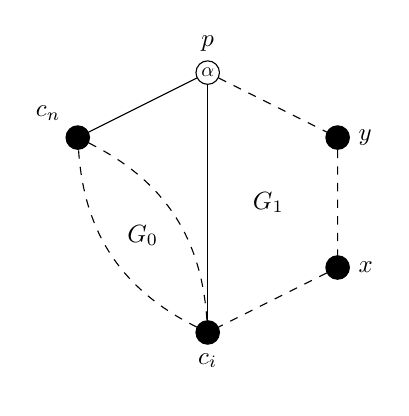
\begin{tikzpicture}[
		scale=1.1,
		every node/.style={circle, draw, minimum size=1mm, scale=0.9},
		every label/.append style={rectangle}
	]
  \node (c_n) [label=above left:$c_n$, fill] at (-1.5cm, 1.25cm) {};
  \node (p) [label=above:{$p$}] at (0cm, 2cm) {};
  \node (p_label) [draw=none, scale=0.8] at (0cm, 2cm) {$\alpha$};
  \node (y) [label=right:$y$, fill] at (1.5cm, 1.25cm) {};
  \node (x) [label=right:$x$, fill] at (1.5cm, -0.25cm) {};
  \node (c_i) [label=below:$c_i$, fill] at (0cm, -1cm) {};
  \node (G_0) [draw=none, ] at (-0.75cm, 0.12cm) {$G_0$};
  \node (G_1) [draw=none] at (0.7cm, 0.5cm) {$G_1$};
  \node (null) [draw=none] at (270:1.5cm) {};
  \draw (c_i) edge [bend left] (c_n) [dashed];
  \draw (c_n) edge [bend left] (c_i) [dashed];
  \draw (c_n) edge (p);
  \draw (p) edge (c_i);
  \draw (p) edge (y) [dashed];
  \draw (y) edge (x) [dashed];
  \draw (x) edge (c_i) [dashed];
\end{tikzpicture}
$\qquad$
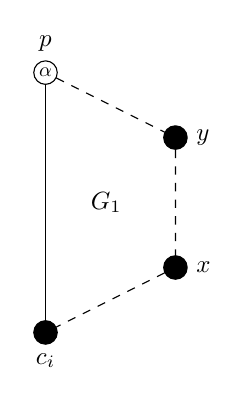
\begin{tikzpicture}[
		scale=1.1,
		every node/.style={circle, draw, minimum size=1mm, scale=0.9},
		every label/.append style={rectangle}
	]
  \node (p) [label=above:{$p$}] at (0cm, 2cm) {};
  \node (p_label) [draw=none, scale=0.8] at (0cm, 2cm) {$\alpha$};
  \node (y) [label=right:$y$, fill] at (1.5cm, 1.25cm) {};
  \node (x) [label=right:$x$, fill] at (1.5cm, -0.25cm) {};
  \node (c_i) [label=below:$c_i$, fill] at (0cm, -1cm) {};
  \node (G_1) [draw=none] at (0.7cm, 0.5cm) {$G_1$};
  \node (null) [draw=none] at (270:1.5cm) {};
  \draw (p) edge (c_i);
  \draw (p) edge (y) [dashed];
  \draw (y) edge (x) [dashed];
  \draw (x) edge (c_i) [dashed];
\end{tikzpicture}
$\qquad$
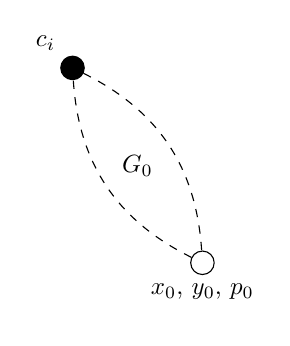
\begin{tikzpicture}[
		scale=1.1,
		every node/.style={circle, draw, minimum size=1mm, scale=0.9},
		every label/.append style={rectangle}
	]
  \node (c_n) [label=above left:$c_i$, fill] at (-1.5cm, 1.25cm) {};
  \node (c_i) [label=below:{$x_0$, $y_0$, $p_0$}] at (0cm, -1cm) {};
  \node (G_0) [draw=none, ] at (-0.75cm, 0.12cm) {$G_0$};
  \node (null) [draw=none] at (270:1.5cm) {};
  \draw (c_i) edge [bend left] (c_n) [dashed];
  \draw (c_n) edge [bend left] (c_i) [dashed];
\end{tikzpicture}
\hfill\\
\footnotesize{\textbf{Figure 3.7} The case $x\ne p$, $y\ne p$, and $c_i\in C[x,p)$.}
\end{center}

\noindent Suppose $x\ne p$, $y\ne p$, and $c_i\in C[x,p)$. In this case $G_1$ must exist, so first apply
the inductive hypothesis to choose $G_1$ from $L$ with $x_1=x$, $y_1=y$, and $p_1=p$.
Since $\alpha\not\in L(v)$ for any $v\in C[x,p)$ we may apply the inductive hypothesis to choose $G_0$ from
$L_0$ with $x_0=y_0=p_0=c_i$. Note that $c_i$ was precolored from our choosing of $G_1$ and recieves
no same color neighbors in $G_0$ so the combined coloring forms a path choosing of $G$ from $L$.\\

\begin{center}
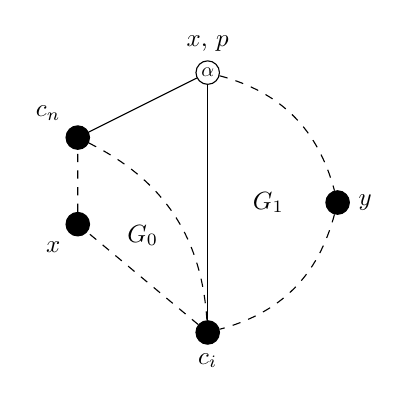
\begin{tikzpicture}[
		scale=1.1,
		every node/.style={circle, draw, minimum size=1mm, scale=0.9},
		every label/.append style={rectangle}
	]
  \node (c_n) [label=above left:$c_n$, fill] at (-1.5cm, 1.25cm) {};
  \node (p) [label=above:{$x$, $p$}] at (0cm, 2cm) {};
  \node (p_label) [draw=none, scale=0.8] at (0cm, 2cm) {$\alpha$};
  \node (x) [label=below left:$x$, fill] at (-1.5cm, 0.25cm) {};
  \node (y) [label=right:$y$, fill] at (1.5cm, 0.5cm) {};
  \node (c_i) [label=below:$c_i$, fill] at (0cm, -1cm) {};
  \node (G_0) [draw=none, ] at (-0.75cm, 0.12cm) {$G_0$};
  \node (G_1) [draw=none] at (0.7cm, 0.5cm) {$G_1$};
  \node (null) [draw=none] at (270:1.5cm) {};
  \draw (c_i) edge (x) [dashed];
  \draw (x) edge (c_n) [dashed];
  \draw (c_n) edge [bend left] (c_i) [dashed];
  \draw (c_n) edge (p);
  \draw (p) edge (c_i);
  \draw (p) edge [bend left] (y) [dashed];
  \draw (y) edge [bend left] (c_i) [dashed];
\end{tikzpicture}
$\qquad$
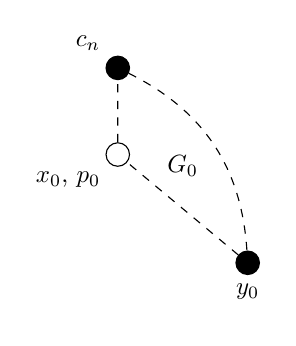
\begin{tikzpicture}[
		scale=1.1,
		every node/.style={circle, draw, minimum size=1mm, scale=0.9},
		every label/.append style={rectangle}
	]
  \node (c_n) [label=above left:{$c_n$}, fill] at (-1.5cm, 1.25cm) {};
  \node (x) [label=below left:{$x_0$, $p_0$}] at (-1.5cm, 0.25cm) {};
  \node (c_i) [label=below:{$y_0$}, fill] at (0cm, -1cm) {};
  \node (G_0) [draw=none] at (-0.75cm, 0.12cm) {$G_0$};
  \node (null) [draw=none] at (270:1.5cm) {};
  \draw (c_i) edge (x) [dashed];
  \draw (x) edge (c_n) [dashed];
  \draw (c_n) edge [bend left] (c_i) [dashed];
\end{tikzpicture}
$\qquad$
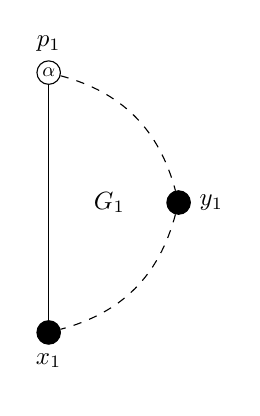
\begin{tikzpicture}[
		scale=1.1,
		every node/.style={circle, draw, minimum size=1mm, scale=0.9},
		every label/.append style={rectangle}
	]
  \node (p) [label=above:$p_1$] at (0cm, 2cm) {};
  \node (p_label) [draw=none, scale=0.8] at (0cm, 2cm) {$\alpha$};
  \node (y) [label=right:$y_1$, fill] at (1.5cm, 0.5cm) {};
  \node (c_i) [label=below:$x_1$,fill] at (0cm, -1cm) {};
  \node (G_1) [draw=none] at (0.7cm, 0.5cm) {$G_1$};
  \node (null) [draw=none] at (270:1.5cm) {};
  \draw (p) edge (c_i);
  \draw (p) edge [bend left] (y) [dashed];
  \draw (y) edge [bend left] (c_i) [dashed];
\end{tikzpicture}
\hfill\\
\footnotesize{\textbf{Figure 3.8} The case $x\ne p$, $y\ne p$, and $c_i\in C(y,x)$.}
\end{center}

\noindent Suppose $x\ne p$, $y\ne p$, and $c_i\in C(y,x)$. In this case $G_1$ must exist. We apply
the inductive hypothesis to color $G_0$ from $L_0$ with $x_0=p_0=x$ and $y_0=c_i$. Then apply the inductive
hypothesis again to choose $G_1$ from $L$ with $x_1=c_i$, $y_1=y$, and $p_1=p$. Notice $c_i$ recieves at most
one same color neighbor in each $G_0$ and $G_1$.\\

\begin{center}
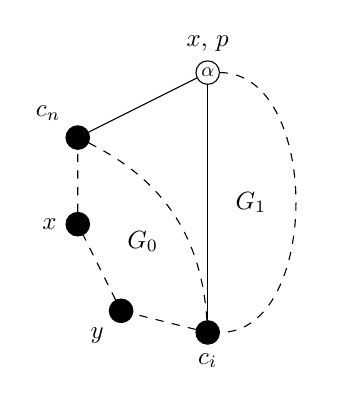
\begin{tikzpicture}[
		scale=1.1,
		every node/.style={circle, draw, minimum size=1mm, scale=0.9},
		every label/.append style={rectangle}
	]
  \node (c_n) [label=above left:$c_n$, fill] at (-1.5cm, 1.25cm) {};
  \node (p) [label=above:{$x$, $p$}] at (0cm, 2cm) {};
  \node (p_label) [draw=none, scale=0.8] at (0cm, 2cm) {$\alpha$};
  \node (x) [label=left:$x$, fill] at (-1.5cm, 0.25cm) {};
  \node (y) [label=below left:$y$, fill] at (-1cm, -0.75cm) {};
  \node (c_i) [label=below:$c_i$, fill] at (0cm, -1cm) {};
  \node (G_0) [draw=none, ] at (-0.75cm, 0.05cm) {$G_0$};
  \node (G_1) [draw=none] at (0.5cm, 0.5cm) {$G_1$};
  \node (null) [draw=none] at (270:1.5cm) {};
  \draw (c_i) edge (y) [dashed];
  \draw (y) edge (x) [dashed];
  \draw (x) edge (c_n) [dashed];
  \draw (c_n) edge [bend left] (c_i) [dashed];
  \draw (c_n) edge (p);
  \draw (p) edge (c_i);
  \draw (p) edge [bend left=90] (c_i) [dashed];
\end{tikzpicture}
$\qquad$
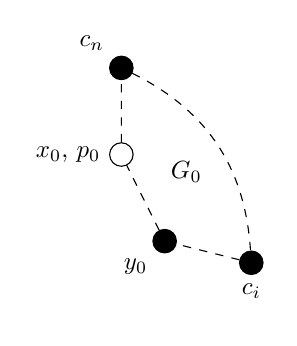
\begin{tikzpicture}[
		scale=1.1,
		every node/.style={circle, draw, minimum size=1mm, scale=0.9},
		every label/.append style={rectangle}
	]
  \node (c_n) [label=above left:{$c_n$}, fill] at (-1.5cm, 1.25cm) {};
  \node (x) [label=left:{$x_0$, $p_0$}] at (-1.5cm, 0.25cm) {};
  \node (y) [label=below left:$y_0$, fill] at (-1cm, -0.75cm) {};
  \node (c_i) [label=below:$c_i$, fill] at (0cm, -1cm) {};
  \node (G_0) [draw=none, ] at (-0.75cm, 0.05cm) {$G_0$};
  \node (null) [draw=none] at (270:1.5cm) {};
  \draw (c_i) edge (y) [dashed];
  \draw (y) edge (x) [dashed];
  \draw (x) edge (c_n) [dashed];
  \draw (c_n) edge [bend left] (c_i) [dashed];
\end{tikzpicture}
$\qquad$
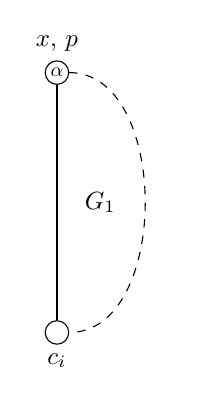
\begin{tikzpicture}[
		scale=1.1,
		every node/.style={circle, draw, minimum size=1mm, scale=0.9},
		every label/.append style={rectangle}
	]
  \node (p) [label=above:{$x$, $p$}] at (0cm, 2cm) {};
  \node (p_label) [draw=none, scale=0.8] at (0cm, 2cm) {$\alpha$};
  \node (c_i) [label=below:$c_i$] at (0cm, -1cm) {};
  \node (G_1) [draw=none] at (0.5cm, 0.5cm) {$G_1$};
  \node (null) [draw=none] at (270:1.5cm) {};
  \draw (p) edge (c_i);
  \draw (p) edge [bend left=90] (c_i) [dashed];
\end{tikzpicture}
\hfill\\
\footnotesize{\textbf{Figure 3.9} The case $x\ne p$, $y\ne p$, and $c_i\in C(p,y]$.}
\end{center}

\noindent Finally, suppose $x\ne p$, $y\ne p$, and $c_i\in C(p,y]$. If
$\alpha\in L(c_i)$ we set $p_0=c_i$ and color $c_i$ with $\alpha$. Otherwise, set $p_0=c_1$ and we color it with
the first color in $L_0(c_1)$, noting $|L_0(c_i)|\ge 2$ in this case. We then apply the inductive hypothesis to
choose $G_0$ from $L_0$ with $x_0=x$, $y_0=y$, and $p_0$. If $G_1$ exists, we then apply the inductive
hypothesis to choose $G_1$ from $L$ with $x_1=p_1=p$ and $y_1=c_i$. Note that $c_i$ was precolored by our
choosing of $G_0$. If $p_0=c_i$ then $c_i$ recieves at most one same
color neighbor in each $G_0$ and $G_1$. If $p_0\ne c_i$, then $y_1=c_i$ is immediatley prior to
$p_1=p$ and thus $c_i$ will recieve no same color neighbors in $G_1$.
\end{proof}

\begin{comment}
\begin{algorithm}
\LinesNumbered
\DontPrintSemicolon
\KwIn{Plane graph $G$ and paths $P=p_0\ldots p_n$ and $Q=q_0\ldots q_m$}
\Begin{
	\Repeat{$t_0\not\in P\cup Q$} {
		$t_0\longleftarrow$ vertex forming face with $p_0$ and $q_0$\;
		\If{$t_0 = p_1$} {
			$P\longleftarrow P - p_0$\;
		}
		\ElseIf{$t_0 = q_1$} {
			$Q\longleftarrow Q - q_0$\; 
		}
	}
	\Repeat{$t_1\not\in P\cup Q$} {
		$t_1\longleftarrow$ vertex forming face with $p_n$ and $q_m$\;
		\If{$t_1 = p_{n-1}$} {
			$P\longleftarrow P - p_n$\;
		}
		\ElseIf{$t_1 = q_{m-1}$} {
			$Q\longleftarrow Q - q_m$\; 
		}
	}
	perform BFS starting at $t_1$\;
	\If{BFS finds $t_0$} {
		$T\longleftarrow$ BFS path $t_0$ to $t_1$\;
	}
	\Else {
		we hit an vertex $u$ with neighbors $p_i\in P$ and $q_j\in Q$\;
		$T\longleftarrow$ BFS path $u$ to $t_1$\;
		recurse on subgraph bounded by $p_0\ldots p_i$ and $q_0\ldots q_j$\;
		$P\longleftarrow p_i\ldots p_n$\;
		$Q\longleftarrow q_j\ldots q_m$\;
	}
	recurse on subgraph bounded by $P$ and $T$\;
	recurse on subgraph bounded by $T$ and $Q$\;
}
\caption{Path 3-Color}
\end{algorithm}
\end{comment}

\section*{References}

\begin{tabularx}{\linewidth}{lX}
[1] & Hartman, C., "Extremal problems in graph theory," Ph.D. thesis, Department of Mathematics,
University of Illinois at Urbana-Champaign, 1997.\\\relax
[2] & Skrekovski, R., "List improper colourings of planar graphs,"
\emph{Combinatorics, Probability and Computing}, vol. 8, pp. 293-299, 1999.\\\relax
[3] & Eaton, N., N. Hull, "Defective list colorings of planar graphs,"
\emph{Bulletin of the Institute for Combinatorics and its Applications}, 1999.\\\relax
[4] & Poh, K., "On the linear vertex-arboricity of a planar graph," \emph{Journal of Graph Theory},
vol. 14, pp. 73-75, 1990\\\relax
[5] & Kant, G., "Algorithms for drawing planar graphs," Ph.D. thesis, Department of Computer Science,
Utrecht University, 1993.\\\relax
[6] & Tarjan, R., "Depth-first search and linear graph algorithms," SIAM Journal on Computing, vol. 1, pp.
146-160, 1972.\\\relax
[6] & Tarjan, R., "Depth-first search and linear graph algorithms," SIAM Journal on Computing, vol. 1, pp.
146-160, 1972.\\\relax
\end{tabularx}

\end{document}